
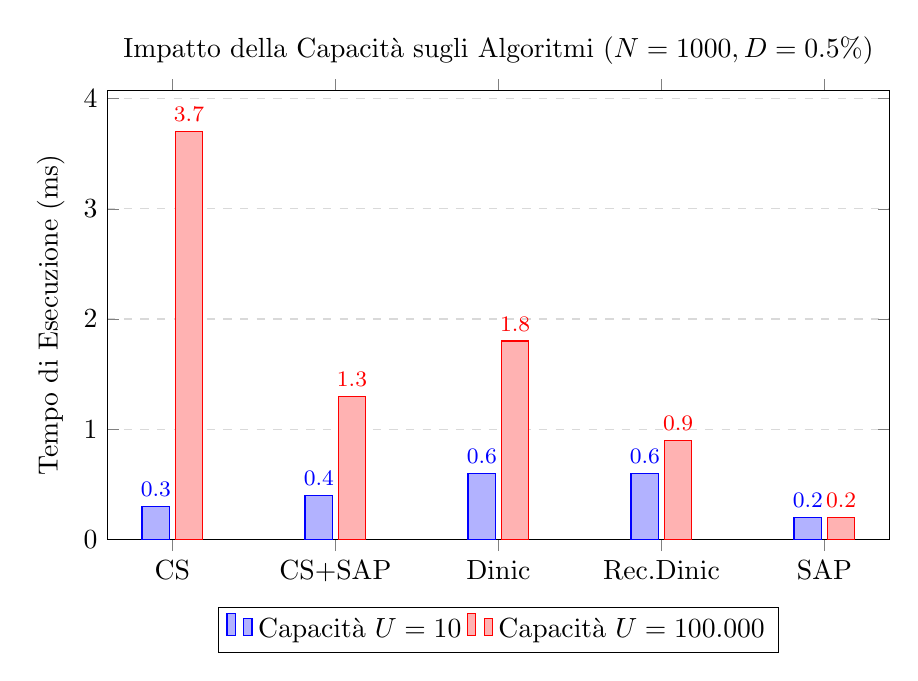
\begin{tikzpicture}
    \begin{axis}[
        ybar,
        title={Impatto della Capacità sugli Algoritmi ($N=1000, D=0.5\%$)},
        width=0.95\textwidth,
        height=0.6\textwidth,
        symbolic x coords={CS,CS+SAP,Dinic,Rec.Dinic,SAP},
        xtick=data,
        ylabel={Tempo di Esecuzione (ms)},
        legend style={at={(0.5,-0.15)}, anchor=north, legend columns=-1},
        ymajorgrids=true,
        grid style={dashed, gray!30},
        nodes near coords,
        nodes near coords style={font=\footnotesize},
        ymin=0
    ]
    \addplot coordinates {(CS, 0.3) (CS+SAP, 0.4) (Dinic, 0.6) (Rec.Dinic, 0.6) (SAP, 0.2) };
    \addlegendentry{Capacità $U=10$}
    \addplot coordinates {(CS, 3.7) (CS+SAP, 1.3) (Dinic, 1.8) (Rec.Dinic, 0.9) (SAP, 0.2) };
    \addlegendentry{Capacità $U=100.000$}

    \end{axis}
\end{tikzpicture}
